



\section{Common Read-out Unit (CRU)}

In order to minimise development and maintenance effort and to simplify system interfaces the ALICE read-out system upgrade is based on the use of a common read-out unit (CRU). Fig.  \ref{fig_ro:cru_block}  shows the block diagram of the module and fig  \ref{fig_ro:cru_photo} shows a photograph. The functionality of the CRU is to provide: 
\begin{itemize}
\item the interface of the sub-detector system via bi-directional optical GBT links to the data read-out in continuous and in triggered mode;
\item the interface to the timing and trigger (TTS) signals provided by the CTP to the detector systems on constant latency links (see measurements in section \ref{sec:ctp_trig_links}). As the FIT and the TOF detector are providing particle arrival measurements the jitter of the timing signals on the path from the machine interface via the CTP and CRU to the detectors has been set to be xxx ps;
\item detector configuration signals from the detector control system (DCS) to the detector systems; 
\item an interface to the first level processor (FLP) in the O2 online/offline system via a PCIe interface;
\item a central firmware frame-work establishing generic data transmission paths between the interfacing components (CTP, FLP, DCS, front-end) including data protocol verification and error reporting to CTP and FLP;
FPGA based processing power for detector specific data processing algorithms such as zero suppression or base-line correction.
\item The CRUs are custom developed, FPGA based, Gen 3 PCI Express plug-in cards installed in the FLPs of the ALICE O2 system. 
\end {itemize} Given similar requirements of the CRU and the PCIe40 card  \cite{ro:PCI40} a development of a custom designed, Gen 3 PCI Express optical link interface card for the LHCb upgrade, ALICE based the CRU development on the same hardware platform and joined the PCIe40 qualification and test effort. The PCIe40 CRU card is based on a state-of-the-art Intel Arria 10 GX FPGA \cite{ro:CRU_FPGA}. Although the hardware is common, the two experiments developed their own firmware versions to fulfil the different functionalities. 

The CRU features up to 48 high-speed, bi-directional, 10 Gb/s optical links using 12-lane Minipod parallel optical transmitters and receivers from Avago/Broadcom \cite{ro:minipods}. These optical links are accessible from the CRU front-panel through MTP optical ribbon cable connectors and establish the interface to the detector front-end electronics using the GBT protocol implemented in the FPGA.
Depending on the operation mode the GBT data links provide a data bandwidth of 4.48 Gb/s in wide-bus mode, or 3.2 Gb/s in GBT mode with forward error correction which provide a superior radiation performance. The number of data links and the use of the forward error correction is adapted to the sub-detector needs. In most cases, 24 data links aggregate the input data into a data stream via the PCIe interface to the FLP servers memories. Table \ref{table_ro:flp} shows the number of CRUs, the number of read-out links and the data throughput into and out of one CRU for each sub-detector.

The bi-directional connection to the 9.6 Gb/s bidirectional TTC-PON network connecting all CRUs to the CTS is established using one out of two SFP+ optical transceivers. These links carry the LHC clock with a jitter below 20 ps rms and transmit the bidirectional trigger and data flow control signals synchronising all 474 CRUs and the connected detectors to each other. 

The 16-lane (x16) PCI Express card edge connector provides the interface between the CRU and the ALICE O2 FLPs, in which the CRUs are installed. Each CRU contains two x8 PCI Express end-points implemented in the Arria 10 FPGA of the card. Through the bifurcation mechanism of the server motherboards, the host computer can handle these end-points as a 16-lane (x16) PCI Express interface. In practice, this interface achieves ~90 Gb/s sustainable data throughput from the CRU to the memory of the FLP computers, see section \ref{sec:jitter_measurments})

The PCIe40 CRU card has an Intel Arria 10 GX main FPGA, type 10AX115S3F45E2SG, and auxiliary components providing on-board power, clock, and configuration management. The cards have on-board high-performance jitter cleaner PLLs to clean the LHC clock received via the optical trigger links from the CTS. 

Power is supplied to the CRUs via their edge connectors and through GPU power cables directly from the server PSU. The FPGA and optical Minipods are cooled using on-board passive heatsinks placed into the forced airflow of the server chassis.   
The received data from the detector links of a CRU are aggregated into a unified data stream and transferred to the memory of the FLPs. The ALICE upgrade foresees sub-detectors  which already prepare data according to the HBF structure in the detector front-end using FPGAs. Other sub-detectors without programmable logic provide a data stream without a HBF structure. For the first group the CRU data aggregation consists of input link data multiplexing. For the second group the CRU provides the HBF structure and compression before forwarding the data to the FLPs. A central FPGA firmware provided by the ALICE CRU design group provides the common interfaces to CTS, FLP, CRU and the sub-detectors. Sub-detector dependent functionality, such as link decoding, adding HBF structure, compression or data processing is added via a dedicated user logic (UL) firmware plug-in to the central FPGA firmware. The UL is provided by the sub-detector groups.

Extract info from Olivier paper about FW design


\begin{figure*}[hbtp]
  \begin{center}
    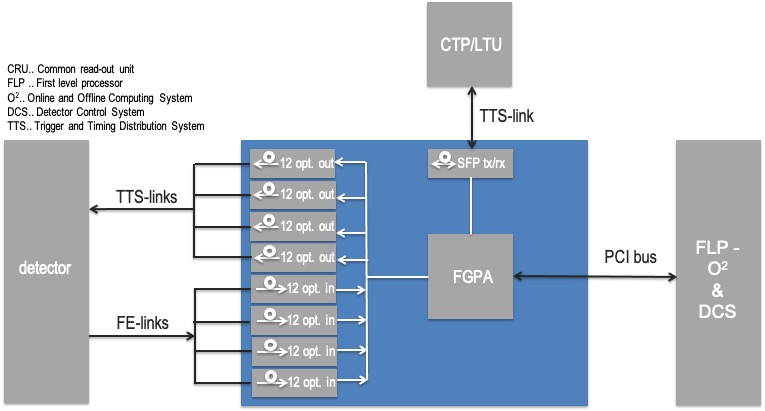
\includegraphics[width=1.\textwidth]{cru/cru_block.jpg}
  \end{center}
  \caption{CRU block diagram}
  \label{fig_ro:cru_block}
\end{figure*}

\begin{figure*}[hbtp]
  \begin{center}
    \includegraphics[width=1.\textwidth]{cru/cru_photo.jpg}
  \end{center}
  \caption{CRU block diagram}
  \label{fig_ro:cru_photo}
\end{figure*}

